\documentclass[11pt, letterpaper]{article}
\usepackage{fullpage}
\usepackage{fancyhdr}
\usepackage[top=2cm, bottom=2cm, left=2cm, right=2cm]{geometry}
\usepackage{lastpage}
\usepackage{enumerate}
\usepackage{amsmath}
\usepackage{mathtools}
\usepackage{textcomp}
\usepackage{enumitem}
\usepackage{tikz}
\usetikzlibrary{automata,positioning}

\newcommand\netid{bvb2}
\newcommand\name{Brock Boehler}
\newcommand\class{ECE 374}
\newcommand\semester{Fall 2019}
\newcommand\Homework{Homework 3}

\pagestyle{fancyplain}
\headheight 30pt
\lhead{\name\\\netid}
\rhead{\class\\\semester}
\chead{\Homework}
\lfoot{}
\rfoot{}
\headsep 10pt

\begin{document}

\section*{Problem 1}
Prove whether the following languages are regular or not.

\begin{enumerate}[label=\Alph*]

\item Strings over the alphabet $\Sigma = \{0,...,9,\#\}$ that contain the substring $c\#^cc$ where $c \in \{0,...,9\} $.

\quad This language \textbf{is} regular - this can be proven by constructing a regular expression that recognizes the language. \textit{(Notation Note: The string $\#^n$ is the string consisting of \# repeated n times. Example: $\#^3 = \#\#\#$)}

$$ \bigcup_{r \in \{0,...,9\}} \Sigma^* (r \#^r r) \Sigma^* $$
$$= \Sigma^*(00)\Sigma^* + \Sigma^*(1\#1)\Sigma^* + ... + \Sigma^*(9\#^9 9)\Sigma^*$$

\quad We have now found a regular expression capturing the language thus proving it is a regular language.

%$$ r = \Sigma^* (00) \Sigma^* + 
%\Sigma^* (1\#1) \Sigma^*  + 
%\Sigma^* (2 \#^2 2) \Sigma^* + 
%\Sigma^* (3 \#^3 3) \Sigma^* +
%\Sigma^* (4 \#^4 4) \Sigma^* + 
%\Sigma^* (5 \#^5 5) \Sigma^* +
%\Sigma^* (6 \#^6 6) \Sigma^* +
%\Sigma^* (7 \$^7 7) \Sigma^* + 
%\Sigma^* (8 \#^8 8) \Sigma^* +
%\Sigma^* (9 \#^9 9) \Sigma^* $$

\item Strings over the alphabet $\Sigma = \{0,...,9,\#\}$ of the form $\langle n \rangle \#^n$ where n is a sequence of digits interpreted as a decimal number.

This language \textbf{is not} regular - this can be proven using fooling sets.

\quad Let us construct a set of strings representing the natural numbers. This is the set of all strings accepted by the regular expression $r_n = (0 + 1 + ... + 9)^+$. This set has countably infinite cardinality as the set of natural numbers has infinite cardinality. This fooling set is distinguishable. We can take any number $n \in r_n$ and attach the suffix of $\#^n$ where n is treated as a number instead of a string. This creates the string $n\#^n$ which is accepted by the aforementioned language, while no other strings in $r_n$ are accepted.

\item Strings over the alphabet $\Sigma = \{0,...,9,\#\}$ that have the same 3 characters repeated in two places.

This language \textbf{is} regular. This can be proven by generating a regular expression that recognizes the language.

\quad Let us begin by defining the regular expression for any string that contains an arbitrary length-3 substring twice. Let the length three substring be denoted '$\alpha \beta \gamma$' such that $\alpha \in \Sigma, \beta \in \Sigma, \gamma \in \Sigma$. We can then take it further and generate a function to generate regular expressions of this type as follows:

$$ r(\alpha, \beta, \gamma) = \Sigma^*(\alpha \beta \gamma) \Sigma^* (\alpha \beta \gamma) \Sigma^* $$

\quad Now that we have the above expression, we can combine all possible combinations of strings with length-3 substrings repeated twice to get the language we set out to prove as regular:

$$ \bigcup_{\alpha \in \Sigma} \bigcup_{\beta \in \Sigma} \bigcup_{\gamma \in \Sigma} r(\alpha, \beta, \gamma) $$
$$ =\Sigma^*(aaa)\Sigma^*(aaa)\Sigma^* + \Sigma^*(aab)\Sigma^*(aab)\Sigma^* + ... + \Sigma^*(zzz)\Sigma^*(zzz)\Sigma^* $$

We have now developed a regular expression for the language of all strings that have a length-3 substring repeated twice, thus proving the language is regular.

\end{enumerate}

\pagebreak

\section*{Problem 2}

\quad Suppose we are given the DFA M such that $M = (\Sigma, Q, s, A, \delta)$ that recognizes the language L and we want to develop an NFA N ( $N = (\Sigma, Q_N, s_N, A_N, \delta_N)$ ) that recognizes $f(L)$. For every $\alpha \in \Sigma$ we can create an NFA that recognizes $f(\alpha)$, which we will denote $N_{f(\alpha)}$. In our original DFA M, we can "cut" each transition line, and replace them in the following way: Take the original source state and connect it to the start state of $N_{f(\alpha)}$ via an epsilon-transition and connect the accepting states of $N_{f(\alpha)}$ to the original destination state via epsilon-transition(s). See the following diagram for a visual representation:

\bigbreak
\begin{center}
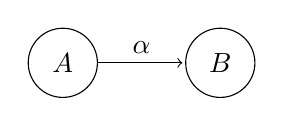
\begin{tikzpicture}[shorten >=1pt,node distance=2cm,on grid,auto]

	\node[state] (A) {$A$};
	\node[state] (B) [right=of A] {$B$};
	\path[->]
	(A) edge node {$\alpha$} (B);

\end{tikzpicture}

\bigbreak
\textit{is transformed into}
\bigbreak

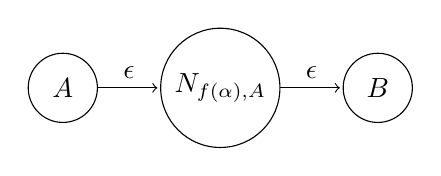
\begin{tikzpicture}[shorten >=1pt,node distance=2cm,on grid,auto]

	\node[state] (A) {$A$};
	\node[state] (F) [right=of A]{$N_{f(\alpha), A}$};
	\node[state] (B) [right=of F] {$B$};
	\path[->]
	(A) edge node {$\epsilon$} (F)
	(F) edge node {$\epsilon$} (B);

\end{tikzpicture}

\end{center}

\quad The accepting states of the new NFA N are the same accepting states of the original DFA M. Another way to describe the change made to recognize $f(L)$ is that for all A, B, and $\alpha$ such that $A \in Q, B \in Q, \alpha \in \Sigma$, if $ \delta(A, \alpha) = B$ then now $B \in \delta_{Nf(\alpha), A}^*(A, \alpha)$. 

To summarize, we construct the NFA to accept $f(L)$ in the following way:

\begin{enumerate}
\item Develop an NFA to recognize each $f(\alpha)$ and ONLY $f(\alpha)$ for each $\alpha$ in $\Sigma$. This is trivial - we can use Thompson's algorithm to develop it. We will call this sub-NFA $N_{f(\alpha)}$
\item Update the delta function of the original DFA M such that if $A \in Q, B\in Q, \alpha \in \Sigma$ and $\delta(A, \alpha) = B$ then now $B \in \delta_{Nf(\alpha), A}^*(A, \alpha)$. Do this for every transition in M, such that now each transition is replaced by a sub-NFA that accepts $f(\alpha)$ and is connected to both the source and destination state of each transition. In other words, $\delta_{Nf(\alpha), A}^*$ is the delta-star function of the sub-NFA $N_{f(\alpha)}$ that connects the state A to other states in the previously mentioned way.
\item $\delta_N^*(q, f(\alpha)) = \delta_{Nf(\alpha), q}^*(q, f(\alpha))$
\item $Q_N = Q \cup (Q \in N_{f(\alpha), A})$ for all $ \alpha \in \Sigma $ and for all $A \in Q$
\item $s_N = s$
\item $A_N = A$
\item $\Sigma_N = \Sigma$
\end{enumerate}

\bigbreak

We will prove that our NFA construction is correct in the following manner: 1. Prove that for every string accepted by DFA M, our NFA accepts the language homomorphism of that string, and 2. For every string rejected by DFA M, the constructed NFA rejects the homomorphism of that string too.

\bigbreak

Prove that for all $x \in L$, the constructed NFA accepts $f(x)$:

\begin{enumerate}

\item Assume we have an arbitrary string $x \in L$ with walk W such that W is the array of states that are visited by the DFA M as the string x is fed through it. We will denote W[0] as the initial starting state, W[1] as the first state visited, and so on until W[E] which is the last state visited. This notation will be applied to x such that x[0] is the initial character, x[1] is the first character, and so on until x[E] which is the last character.
\item The starting state of NFA N is the same as the starting state of DFA M
\item We begin by feeding our NFA N the sub-string $f(x[0])$. 
\item $f(x[0])$ is accepted by the sub-NFA $N_{f(x[0]),s}$.
\item This process can be repeated recursively for each character $x[n] \in x$. We plug in $f(x[n])$ into our delta function, and now W[n] is a state we are currently visiting in N. This is due to the definition of our delta function for N
\item This process is repeated until all x[n] are exhausted. When we finish processing x, we will have arrived at an accepting state due to the previous point.
\item Therefore, if x is accepted by M, then $f(x)$ will be accepted by N. This is because if M ends on W[n] while processing x, then our NFA N will also end on W[n] while processing $f(x)$.

\end{enumerate}

\bigbreak

Prove that for all $x \notin L$ the constructed NFA rejects $f(x)$:

\begin{enumerate}
\item From the previous proof we have shown that besides visiting the sates of the sub-NFA's connecting states, if we input $f(x)$ into N, then we visit the same states as we do in DFA M.
\item Therefore, if we visit the same states, our walk will end on the same state in N as it does in M.
\item If x ends on a non accepting state in M, then $f(x)$ will end in the same non accepting state in N, meaning it will also not be accepted by N.
\end{enumerate}

We have now shown that our construction of N is correct and if x is accepted by M, then N will accept $f(x)$. If x is rejected by M, then $f(x)$ will also be rejected by N.

\pagebreak

\section*{Problem 3}

\begin{enumerate}[label=\Alph*]

\item Binary strings that have remainder 2 when divided by 5.

We can define the CFL as follows, with $R_2$ being the nonterminal that represents the language:

\begin{center}
\begin{tabular}{l}
$R_2 = R_1 0\ |\ R_3 1 $ \\
$R_0 = R_0 0\ |\ R_2 1 $ \\
$R_1 = R_0 1\ |\ R_3 0\ |\ 1 $ \\
$R_3 = R_1 1\ |\ R_4 0 $ \\
$R_4 = R_2 0\ |\ R_4 1 $ \\
\end{tabular}
\end{center}

\quad Where $R_n$ represents the language of binary strings such that $mod_5(R_n) = n$. The above table holds true because of what happens whenever you add a 1 or 0 to the end of a binary string. Suppose we have a number that is of the form $5N + M$ where M is strictly less than 5. This means that $mod_5(5N + M) = M$. When we add a 0 to the end of this string, it is equivalent to doing: $ 2 * (5N + M) + 0 = 10N + 2M \implies mod_5(10N + 2M) = mod_5(2M)$. Adding a 1 to the zero is equivalent of doing: $ 2 * (5N + M) + 1 = 10N + 2M + 1 \implies mod_5(10N + 2M + 1) = mod_5(2M+1)$. 

\quad Because we know what the remainder of each language is currently, we can predict what the remainder will be after appending a 1 or 0. This allows us to construct nonterminal languages that represent strings with specific remainders and allow  us to create a CFL with their relations.

\item Strings over the alphabet $\{0, 1\}$ that have two blocks of 0's of equal length.

We can define the CFL as follows, with C being the nonterminal that represents the desired language.

\begin{center}
\begin{tabular}{l}
$C = EAFAB $\\
$A = 0\ |\ 0A$ \\
$D = \epsilon\ |\ 0\ |\ 0D\ |\ 1D $ \\
$E = \epsilon\ |\ D1 $ \\
$F = 1\ |\ 1D1 $ \\
$B = \epsilon\ |\ 1D $ \\

\end{tabular}
\end{center}

\quad The nonterminals are defined as follows:
\begin{itemize}

\item C is the desired language of all strings containing two blocks of equal-length 0's. We have E which is either nothing or a string ending in 1, followed by a block of zero's, followed by either a single 1 or a string beginning and ending with 1, followed by an equal-lengh block of 0's, followed by either nothing or a string beginning in 1.

\item A is an arbitrary-length string of only 0's

\item D is any possible string made out of 0 or 1's

\item E is either an empty string or a string ending in 1. We can take any arbitrary string and put a 1 at the end to enforce it ends in 1

\item F is any string that begins and ends with 1 or simply the string '1'. We can take any arbitrary string and put 1's at the beginning and end to enforce it begins and ends with 1.

\item B is either an empty string or a string that ends in 1. We can take any arbitrary string and put 1 at the end to enforce that it ends in 1.

\end{itemize}

\pagebreak

\item Arithmetic expressions over decimal numbers using the addition, multiplication, and exponentiation with minimal parenthesis.

We can define the CFL as follows, with E being the nonterminal that represents the desired language

\begin{center}
\begin{tabular}{l}

$E = N\ |\ A\ |\ M\ |\ X\ |\ E + A\ |\ E+M\ |\ E+X $ \\
$N = \{0,...,9\}\ |\ NN $ \\
$A = N + N\ |\ A + N\ |\ M+M\ |\ A+M\ |\ M+A$ \\
$M = N*N\ |\ N*(A)\ |\ (A)*N\ |\ (A)*(A)\ |\ M*M\ |\ M*X\ |\ X*M $ \\
$X = N^N\ |\ (M)^N\ |\ (A)^N\ |\ (X)^N $ \\

\end{tabular}
\end{center}

\quad The nonterminals are defined as follows:

\begin{itemize}

\item E is the language of all arithmetic expressions that follow the aforementioned rules. This can be a single number, an addition term, a multiplication term, or some combination thereof. Because we know each M, X, and A term follows the desired rules, we can rest assured that when we add them together they'll still follow the rules.

\item N is the language of all natural numbers. We can start off with any one of the numbers between 0 to 9, or we can add a digit to the end to create a larger number. Note: N contains numbers with leading 0's (such as 007 = 07 = 7). This is acceptable because even with the trailing 0's the number is still correct.

\item A is the language of select addition terms, this can be addition between two or more numbers, or the addition between two multiplication terms. A can be addition between two terms (N+N), three or more terms (A+N), or between two multiplication terms (M+M), or a series of numbers or a multiplication term plus an addition term (A+M). This is important because it allows us to consolidate terms which can then be wrapped in parenthesis and be multiplied or exponentiated without violating rules

\item M is the language of addition terms, which can be between two or three numbers, two addition terms, or two multiplication terms. M can be two numbers multiplied, an addition term multiplied, two addition terms multiplied together, a multiplication term times an exponentiation term, or two multiplication terms multiplied together. We know that A will be two or more terms added together, so we can wrap the A term's in parenthesis and be ensured the resulting expression follows the rules.

\item X is the language of exponentiation terms, which can be a number to a power, a multiplication term to a higher power, an addition term to a higher power, or an exponentiation term to a higher power. We can add parenthesis around the M, A, and recursive X term and be ensured that the resulting expression follows the rules.

\end{itemize} 

\end{enumerate}

\end{document}